\renewcommand*{\arraystretch}{1.1}

\subsection*{Interactive / update / 4}
\label{sec:interactive-update-04}

\noindent\begin{tabularx}{\queryCardWidth}{|>{\queryPropertyCell}c|X|}
	\hline
	query & Interactive / update / 4 \\ \hline
%
	title & Add Forum \\ \hline
%
    pattern & \hfill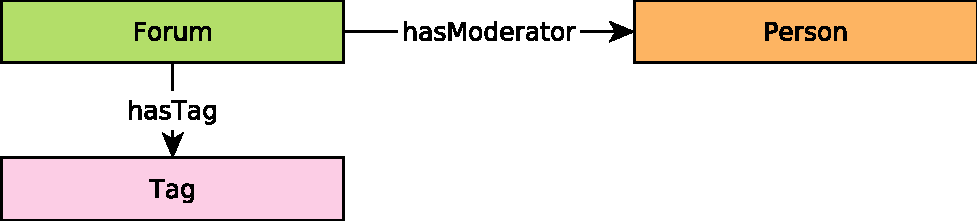
\includegraphics[scale=\patternscale,margin=0cm .2cm]{patterns/interactive-update-04}\hfill\vadjust{} \\ \hline
%
	desc. & Add a Forum to the social network.
 \\ \hline
%
	
%
    
        params &
        \innerCardVSpace{\begin{tabularx}{\attributeCardWidth}{|>{\paramNumberCell}c|>{\varNameCell}M|>{\typeCell}m{\typeWidth}|Y|} \hline
        \cellcolor{parameter} \color{white} \footnotesize $\mathsf{1}$ &Forum.id& ID &  \\ \hline
        \cellcolor{parameter} \color{white} \footnotesize $\mathsf{2}$ &Forum.title& String &  \\ \hline
        \cellcolor{parameter} \color{white} \footnotesize $\mathsf{3}$ &Forum.creationDate& DateTime &  \\ \hline
        \cellcolor{parameter} \color{white} \footnotesize $\mathsf{4}$ &Forum-hasModerator->Person.id& ID &  \\ \hline
        \cellcolor{parameter} \color{white} \footnotesize $\mathsf{5}$ &Forum-hasTag->Tag.id& \{ID\} &  \\ \hline
        \end{tabularx}}\innerCardVSpace \\ \hline
	
%
	
%
	%
	%
	%
    %
\end{tabularx}
\queryCardVSpace